\documentclass[12pt,a4paper]{article}
\usepackage{comment}
\usepackage[hidelinks]{hyperref}
\usepackage{listings}
\usepackage{graphicx}
\graphicspath{{../Data_modelling/Assets}}

\usepackage{subcaption}
\usepackage{float}
\usepackage[table,xcdraw]{xcolor}
\usepackage{wrapfig}

\usepackage{xcolor}

\definecolor{codegreen}{rgb}{0,0.6,0}
\definecolor{codegray}{rgb}{0.5,0.5,0.5}
\definecolor{codepurple}{rgb}{0.58,0,0.82}
\definecolor{backcolour}{rgb}{0.95,0.95,0.92}

\lstdefinestyle{mystyle}{
    backgroundcolor=\color{backcolour},   
    commentstyle=\color{codegreen},
    keywordstyle=\color{magenta},
    numberstyle=\tiny\color{codegray},
    stringstyle=\color{codepurple},
    basicstyle=\ttfamily\footnotesize,
    breakatwhitespace=false,         
    breaklines=true,                 
    captionpos=b,                    
    keepspaces=true,                 
    numbers=left,                    
    numbersep=5pt,                  
    showspaces=false,                
    showstringspaces=false,
    showtabs=false,                  
    tabsize=2
}

\lstset{style=mystyle}

\title{%
    \vspace*{-5mm}\Huge GW2-SRS DATA MODELLING \\
    \vspace*{2mm}\Large powered by \LaTeX}

\author{\vspace*{-5mm}\large Daniel Lopez: \textbf{Data Modelling}}

\begin{document}
    
    \maketitle

    \begin{figure}[H]
        \centering
        
\includegraphics[width=1 \textwidth]{Images/Nuevo_logo_GW2.png}
    \end{figure}

    \newpage

    \section*{4.0 DATA MODELLING}

    \section*{\large 4.1 Introduction}
    \subsection*{\normalsize 4.1.1 Dates and Data}
    All the data used in this study is based on the class performance between May and September. This means
    that, with future nerfs and buffs to classes, values can easily vary. Therefore, this information is only
    relevant in those months. Nonetheless, some classes does not change a lot, so not every value has a chance
    to change.\\

    \subsection*{\normalsize 4.1.2 Model explanation}
    This project data was easier to store on MongoDB than it was on SQL, therefore, a data model was needed not
    only to connect data between tables, but also to have a data schema and keep everything ordered.

    The basic structure of data on MongoDB was explained on the previous EXTRACT part, as the info was saves with
    that specific schema. In SQLite, I needed to create several tables:

    \begin{itemize}
        \item Player's info
        \item Boss names
        \item Profession names
        \item DPS Tables for each boss
    \end{itemize}
    
    \bigskip

    The first table in the list contains names, accounts and two more columns, one of the columns contains a Foreign
    Key (\textbf{FK}) that connects to Boss Names by its Primary Key (\textbf{PK}), as for the second one, it
    contains another FK that connects to Profession names PK. Boss Names and Profession Names are two tables that
    only contains a PK and the names respectively. This was designed this way to prevent data repeating over and over
    when using a PK and FK was by far, the best option.

    \newpage

    Inside the DPS Tables, I had quite a few problems linking data between tables. The DPS tables stored data based 
    on an ID as well, but if \textit{JohnDoe.9100} had ID 30 on the players table and his damage in Vale Guardian corresponds 
    to ID 2 it wouldn't work at all, there was no connection and therefore it leads to error.\\

    The solution was not what I would have done if I had other options in mind, however, it worked fine. I created a FK 
    for every dps table that contained the user account, this way we could just refer the FK to the players table and get 
    the connection done. I thought on doing it with the boss number, but it could also resulted in some problems.

    This choice was mainly done because we use ID as a unique value that represents something, and actually, in a game, your 
    account name is already a unique value that identifies the player and it's also \textbf{immutable}.

    \section*{\large 4.2 Results, Graphs and Analysis}
    The analysis on the project has two main objectives:

    \begin{itemize}
        \item Profession/Class Usage per boss
        \item DPS done per class on each boss
    \end{itemize}

    \bigskip

    \subsection*{\normalsize 4.2.1 Profession/Class Usage}

    \begin{figure}[h!]

        \centering

        \begin{subfigure}{0.5\textwidth}
            \centering
            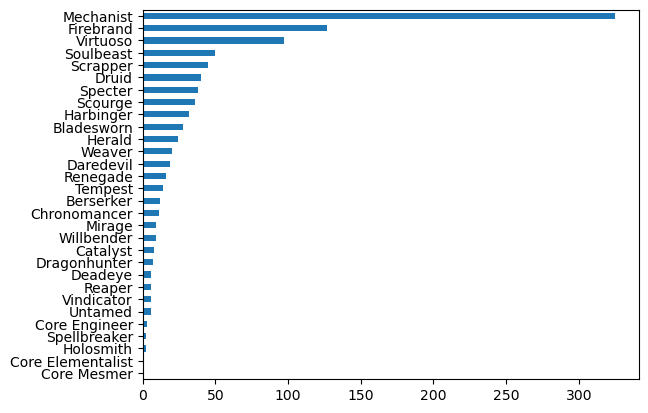
\includegraphics[scale=0.4]{vg_graph.png}
            \caption{\small W1: Vale Guardian Graph}
        \end{subfigure}%
        \begin{subfigure}{0.5\textwidth}
            \centering
            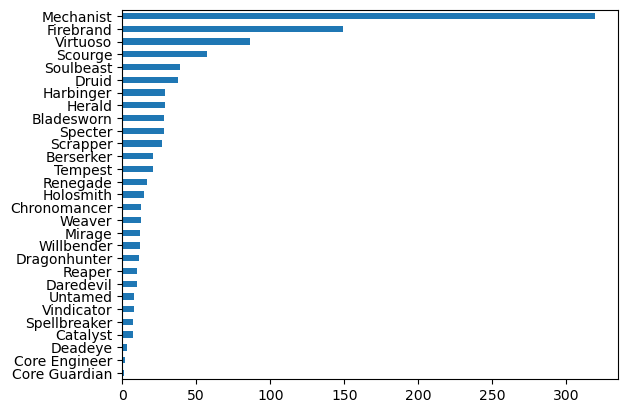
\includegraphics[scale=0.4]{gors_graph.png}
            \caption{\small W1: Gorseval Graph}
        \end{subfigure}
    \end{figure}

    \newpage

    \begin{figure}[h!]

        \centering

        \begin{subfigure}{0.5\textwidth}
            \centering
            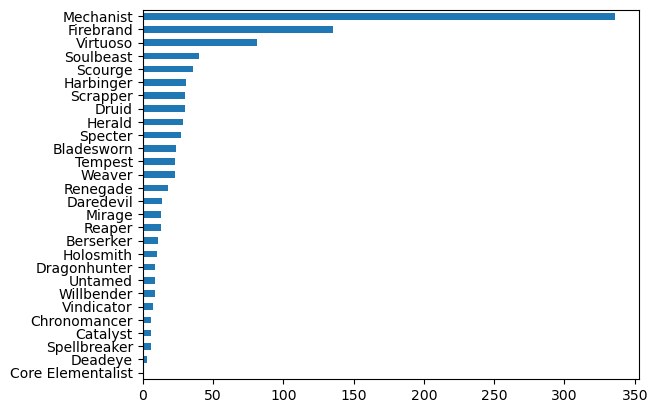
\includegraphics[scale=0.4]{sab_graph.png}
            \caption{\small W1: Sabetha Graph}
        \end{subfigure}%
        \begin{subfigure}{0.5\textwidth}
            \centering
            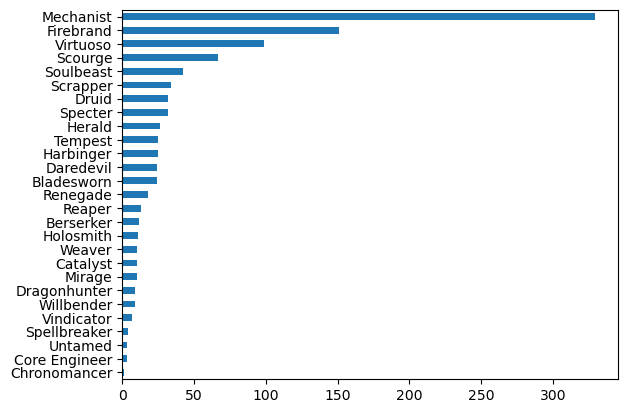
\includegraphics[scale=0.4]{sloth_graph.png}
            \caption{\small W2: Slothasor Graph}
        \end{subfigure}

        \begin{subfigure}{0.5\textwidth}
            \centering
            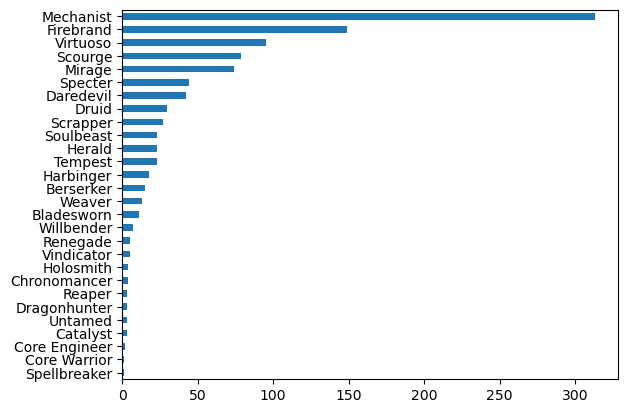
\includegraphics[scale=0.4]{matt_graph.png}
            \caption{\small W2: Matthias Gabrel Graph}
        \end{subfigure}%
        \begin{subfigure}{0.5\textwidth}
            \centering
            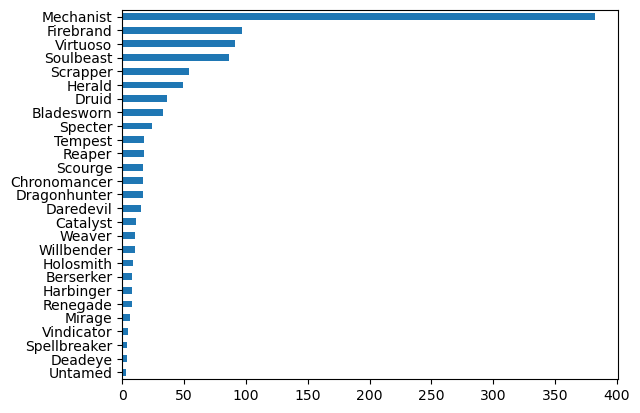
\includegraphics[scale=0.4]{kc_graph.png}
            \caption{\small W3: Keep Construct Graph}
        \end{subfigure}

        \begin{subfigure}{0.5\textwidth}
            \centering
            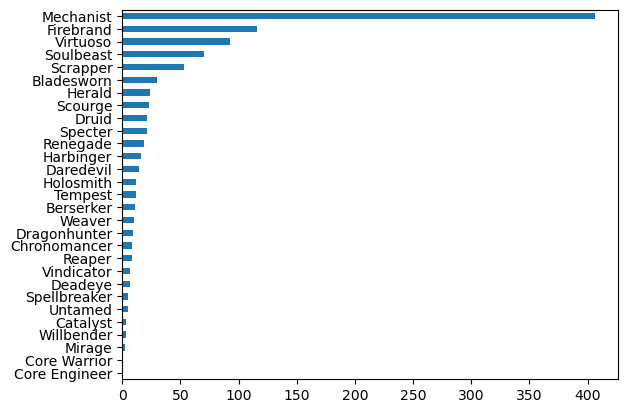
\includegraphics[scale=0.4]{xera_graph.png}
            \caption{\small W3: Xera Graph}
        \end{subfigure}%
        \begin{subfigure}{0.5\textwidth}
            \centering
            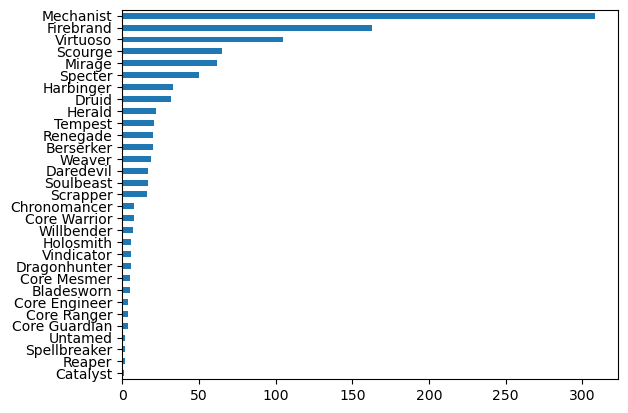
\includegraphics[scale=0.4]{cairn_graph.png}
            \caption{\small W4: Cairn Graph}
        \end{subfigure}

        \begin{subfigure}{0.5\textwidth}
            \centering
            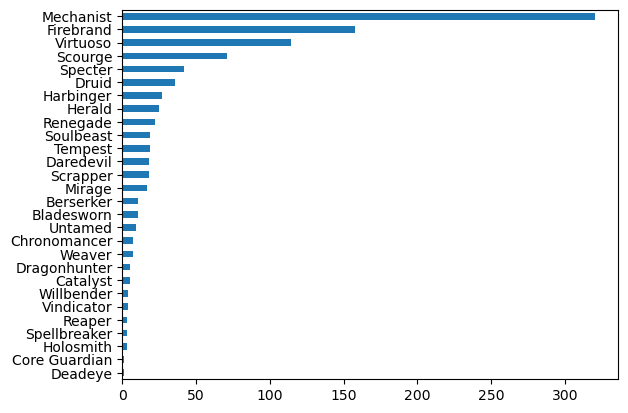
\includegraphics[scale=0.4]{mo_graph.png}
            \caption{\small W4: Mursaat Graph}
        \end{subfigure}%
        \begin{subfigure}{0.5\textwidth}
            \centering
            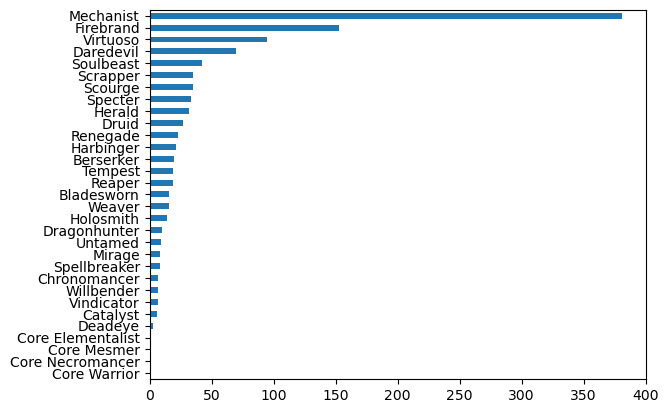
\includegraphics[scale=0.4]{sam_graph.png}
            \caption{\small W4: Samarog Graph}
        \end{subfigure}
    \end{figure}

    \newpage

    \begin{figure}[h!]
        
        \centering

        \begin{subfigure}{0.5\textwidth}
            \centering
            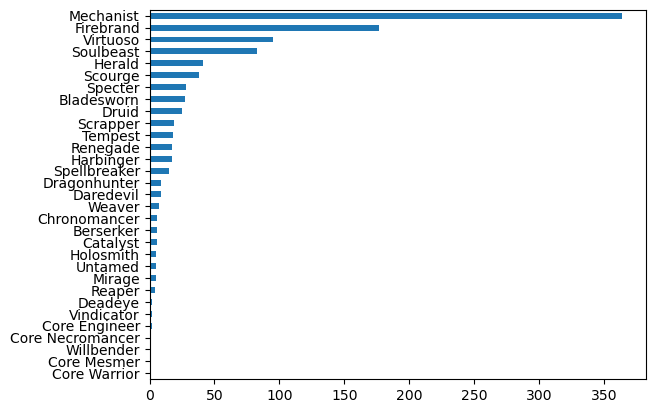
\includegraphics[scale=0.4]{dei_graph.png}
            \caption{\small W4: Deimos Graph}
        \end{subfigure}%
        \begin{subfigure}{0.5\textwidth}
            \centering
            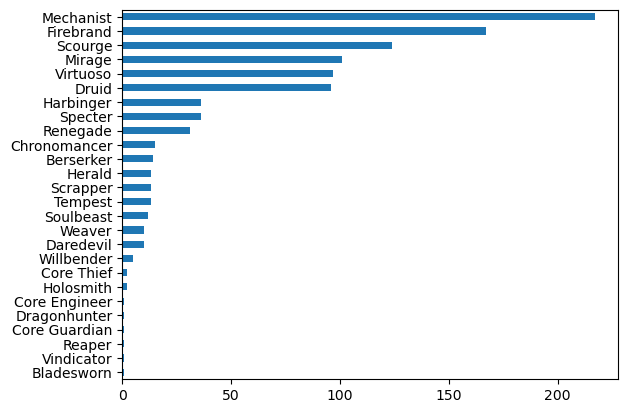
\includegraphics[scale=0.4]{sh_graph.png}
            \caption{\small W5: Soulless Horror Graph}
        \end{subfigure}

        \begin{subfigure}{0.5\textwidth}
            \centering
            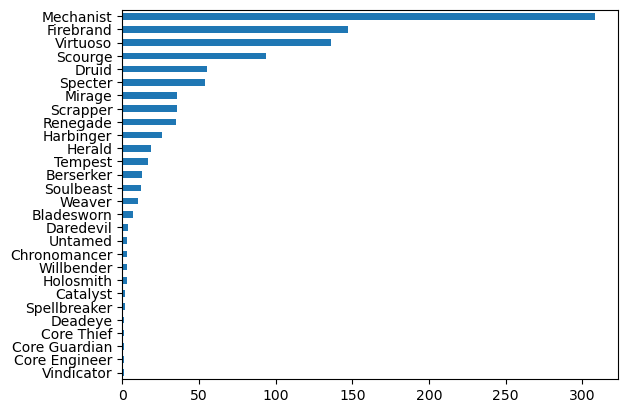
\includegraphics[scale=0.4]{dhuum_graph.png}
            \caption{\small W5: Dhuum Graph}
        \end{subfigure}%
        \begin{subfigure}{0.5\textwidth}
            \centering
            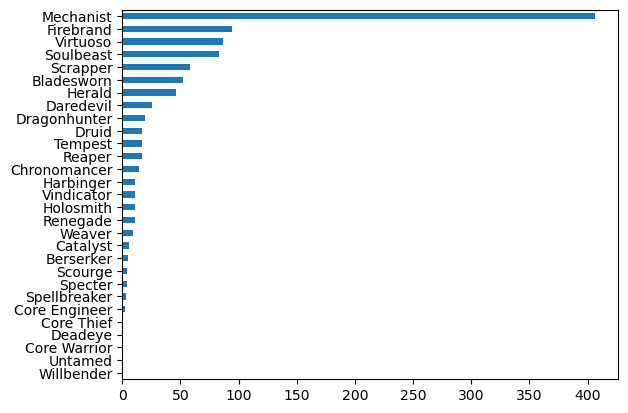
\includegraphics[scale=0.4]{ca_graph.png}
            \caption{\small W6: Conjured Amalgamate Graph}
        \end{subfigure}

        \begin{subfigure}{0.5\textwidth}
            \centering
            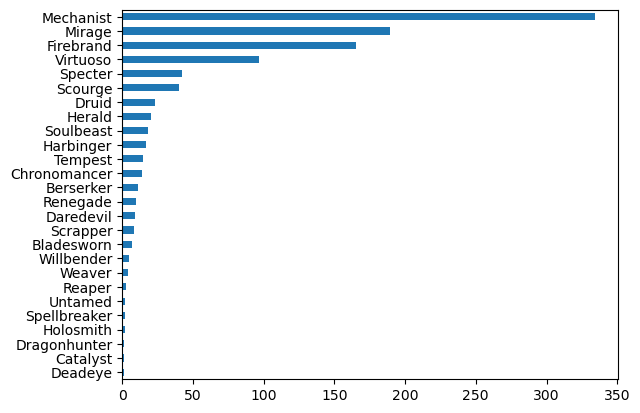
\includegraphics[scale=0.4]{twins_graph.png}
            \caption{\small W6: Twin Largos Graph}
        \end{subfigure}%
        \begin{subfigure}{0.5\textwidth}
            \centering
            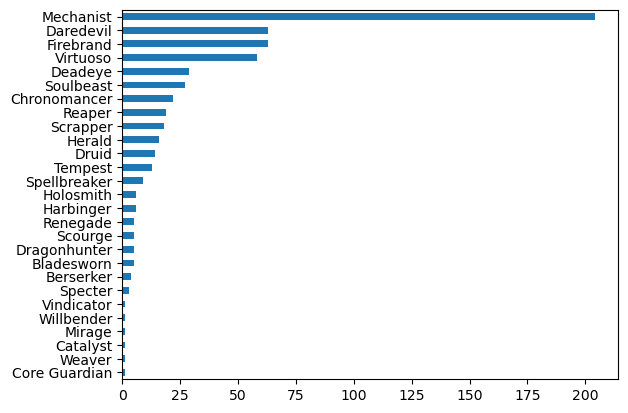
\includegraphics[scale=0.4]{q1_graph.png}
            \caption{\small W6: Qadim Graph}
        \end{subfigure}

        \begin{subfigure}{0.5\textwidth}
            \centering
            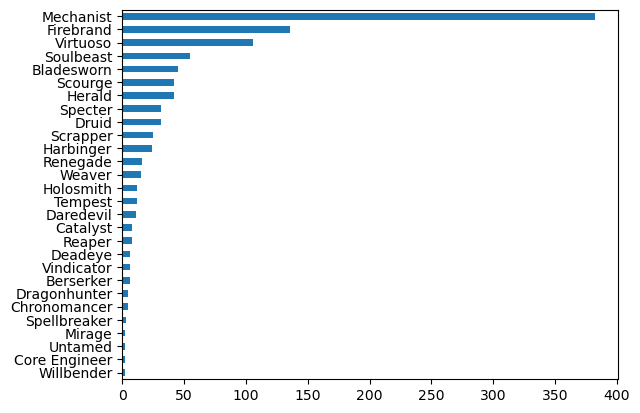
\includegraphics[scale=0.4]{adina_graph.png}
            \caption{\small W7: Cardinal Adina Graph}
        \end{subfigure}%
        \begin{subfigure}{0.5\textwidth}
            \centering
            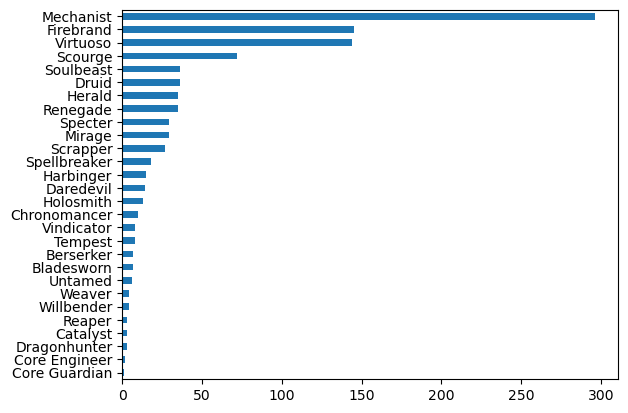
\includegraphics[scale=0.4]{sabir_graph.png}
            \caption{\small W7: Cardinal Sabir Graph}
        \end{subfigure}
    \end{figure}

    \newpage

    \begin{wrapfigure}{r}{0.5\textwidth}
        \centering
        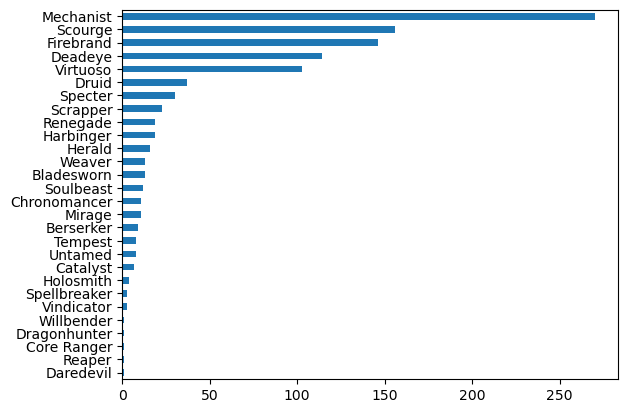
\includegraphics[scale=0.4]{prlqadim_graph.png}
        \caption{\small W7: Peerless Qadim Graph}
    \end{wrapfigure}

    All this graphs represent the class usage in each boss, and it stands out that the usage of
    the Mechanist class is huge. Just to be clear, \textbf{all this analysis is made from data 
    between May and September 2022}, therefore, during this period, Mechanist was a rather new 
    class since Guild Wars 2: End of Dragons came out in February 2022.\\

    Since the release of the Mechanist, as well as other classes, it became one of the best choices
    because it could be either support or dps, and it's results in raid were extremely good. We can 
    also see that other classes such as Firebrand is also quite high on the graph, and this is also
    due to Firebrand's versatility. Guild Wars 2 is a game where versatility in terms of raid and 
    fractals is really important, abilities that can provide \textbf{aegis}, \textbf{alacrity} and 
    \textbf{quickness} are three of the key support buffs, while \textbf{power} and \textbf{fury}
    are two of the key damage buffs. This is why classes like Guardian and Engineer are always on 
    top of the usage graphs.\\

    Each boss also has certain classes that perform better than others, as some bosses are weaker to
    condition damage and other bosses to power damage. On top of that, each boss also has certain
    mechanics, which normally needs certain classes to perform those specific roles; as an example,
    Peerless Qadim has the \textbf{Pylon} mechanic, and it's normally performed by Deadeyes or Scourges.

\end{document}